\chapter{Opis badania}\label{chapter:opis_badania}

\section{Cel i metodologia badań}\label{chapter:cel_i_metodologia_badan}

Przeprowadzenie odpowiednich badań jest kluczowym elementem pracy, który ma na celu znaczące wsparcie odpowiedzi na postawione pytania badawcze.
Po pierwsze, skupiono się na dwóch pierwszych pytaniach badawczych:
\begin{itemize}
    \item PB1: Które metody optymalizacji pozwalają na najlepszą poprawę czasu wykonania funkcji AWS Lambda w ekosystemie Java?
    \item PB2: W jakim stopniu wybrane metody optymalizacji redukują czas zimnego startu funkcji Java w AWS Lambda?
\end{itemize}
Aby udzielić odpowiedzi na powyższe pytania, zdecydowano się na wykonanie testów wydajnościowych funkcji.
Opierały się one na przygotowanych wcześniej funkcjach, które implementowały konkretne metody optymalizacji (opisane w Rozdziale \ref{chapter:wybrane_metody_optimalizacji}).
Specyfikacja poszczególnych funkcji została przedstawiona w kolejnych rozdziałach.
Bazując na wnioskach wyciągniętych w ramach przeglądu literatury (opisanego w Rozdziale \ref{chapter:przeglad_literatury}) zdecydowano się na rozszerzenie badania o wybrane parametry, które mogą wpłynąć na ogólną wydajność usługi.
Były to wielkość pamięci funkcji oraz pomiar zarówno ciepłych, jak i zimnych startów.  

W celu porównania skuteczności wybranych metod opracowano konkretne metryki, które zostały użyte w badaniu:
\begin{enumerate}
    \item Czas działania funkcji podczas ciepłego startu (w milisekundach).
    \item Czas działania funkcji podczas zimnego startu (w milisekundach).
    \item Współczynnik wydajności funkcji.
    \item Koszt działania funkcji (w dolarach amerykańskich).
\end{enumerate}

Pierwsza metryka, czyli czas działania funkcji podczas ciepłego startu jest najprostszym pomiarem.
Określa ona bezpośrednio wydajność funkcji w przypadku większości wywołań.
Dlatego metryka ta pełni kluczową rolę w określeniu efektywności poszczególnych metod.
Aby jednak zawrzeć w badaniu także drugi rodzaj startów (oraz odpowiedzieć na drugie pytanie badawcze), określono kolejną metrykę, czyli czas działania funkcji podczas zimnego startu.
W celu dokonania jego pomiaru, niezbędne jest odpowiednie przygotowanie funkcji, które wymaga większych nakładów pracy w przygotowaniu środowiska badawczego, co zostało opisane w kolejnych rozdziałach.
Pozwala to jednak na rzetelniejsze określenie skuteczności konkretnych metod.
Same zimne starty są uznawane za problematyczne w przypadku użycia Javy w AWS Lambda \cite{9284261}\cite{8605777}.
Dlatego metryka ta jest wymagana, by ująć w badaniu bardziej rzeczywiste przypadki użycia usługi.

Osobna analiza ciepłych i zimnych startów jest jednak niewystarczająca, aby rzetelnie określić efektywność metod w kontekście ich praktycznego użycia.
W momencie działania, funkcje AWS Lambda doświadczają obu typów startów, z dominacją ciepłych startów w przypadku aktywnych funkcji.
Z tego powodu rozszerzono badania o metryki, na które wpływ ma czas działania funkcji podczas obu wariantów uruchomień.
Są to współczynnik wydajności funkcji oraz koszt jej działania.

Na potrzeby pracy został zaproponowany współczynnik wydajności funkcji (WWF). 
Wpływ na niego mają zarówno ciepłe, jak i zimne uruchomienia funkcji.
Aby opracowany współczynnik lepiej odwzorowywał realne użycie usługi AWS Lambda zdecydowano się na wykorzystanie wag, które modyfikują oddziaływanie ciepłych i zimnych startów.
Możliwe jest porównanie skuteczności metod optymalizacji wydajności poprzez porównanie wartości WWF, gdzie im wyższa wartość, tym efektywniejsza jest dana metoda.
Współczynnik wydajności funkcji określony jest wzorem:

\[
\mathrm{WWF} = \frac{1000}{t_c \cdot w_c + t_w \cdot w_w}
\]

gdzie:
\begin{itemize}
  \item \( t_c \) - średni czas zimnego startu funkcji [ms],
  \item \( t_w \) - średni czas ciepłego startu funkcji [ms],
  \item \( w_c \) - waga zimnych startów,
  \item \( w_w \) - waga ciepłych startów.
\end{itemize}

Kolejną metryką łączącą ciepłe i zimne starty jest koszt działania funkcji.
Jest to jeden z głównych elementów wdrożenia technologii bezserwerowych, które rozliczane są w zależności od użycia usług.
W przypadku AWS Lambda jest on określany ze względu na czas działania funkcji, wielkość pamięci oraz liczbę wywołań \cite{awsLambdaPricing}.
Ostatni czynnik nie został zawarty w metryce, gdyż nie jest on zależny od wydajności funkcji.
Dwa pierwsze liczone są jako GB-sekundy, które są iloczynem wielkości pamięci (w GB) i czasu działania funkcji (w sekundach).
Metryka ta jest istotna, gdyż w badaniu zostały zawarte różne wielkości pamięci funkcji.
Z tego względu wartościowy jest także pomiar wpływu poszczególnych metod na wydajność kosztową, na którą składają się zarówno czas działania, jak i wielkość pamięci.
Na potrzeby pracy koszt działania przykładowej funkcji został określony wzorem:

\[
\text{K} = P \cdot M \cdot  r \cdot \left( p_c \cdot d_c + p_w \cdot d_w \right)
\]

gdzie:
\begin{itemize}
  \item \( K \) - całkowity koszt działania funkcji [USD],
  \item \( P \) - cena za jedną GB-sekundę [USD],
  \item \( M \) - pamięć funkcji [GB],
  \item \( r \) - liczba wywołań funkcji na sekundę,
  \item \( p_w \) - udział ciepłych startów (np. 0,95),
  \item \( p_c \) - udział zimnych startów (np. 0,05), gdzie \( p_c = 1 - p_w \),
  \item \( d_c \) - średni rozliczany czas dla zimnych startów (w sekundach),
  \item \( d_w \) - średni rozliczany czas dla ciepłych startów (w sekundach).
\end{itemize}

% TODO: opisać badanie w związku z PB3 (czas budowy, dostępność SDK, wielkość artefaktu (?), wsparcie dla testów (?))

\section{Implementacja funkcji}\label{chapter:implementacja_funkcji}

% Co robi funkcja? Dlaczego taka, dlaczego nie używa usług zewnętrznych
% Co dokładnie zaimplementowano: Java (Quarkus + GraalVM), Kotlin (CommonMain + odpowiednio JVM, Native, JS) oraz SnapStart
% Jakieś problemy, które są związane z implementacją (np. funkcja async dla KotlinJS, budowa Kotlin/Native)

\section{Wdrożenie funkcji}\label{chapter:implementacja_funkcji}

% Opisać cały proces budowy z użyciem githuba i wrzucaniem na S3
% Opisać proces wdrażania z terraformem

\section{Środowisko badawcze}\label{chapter:implementacja_funkcji}

\begin{figure}[h]
    \centering
    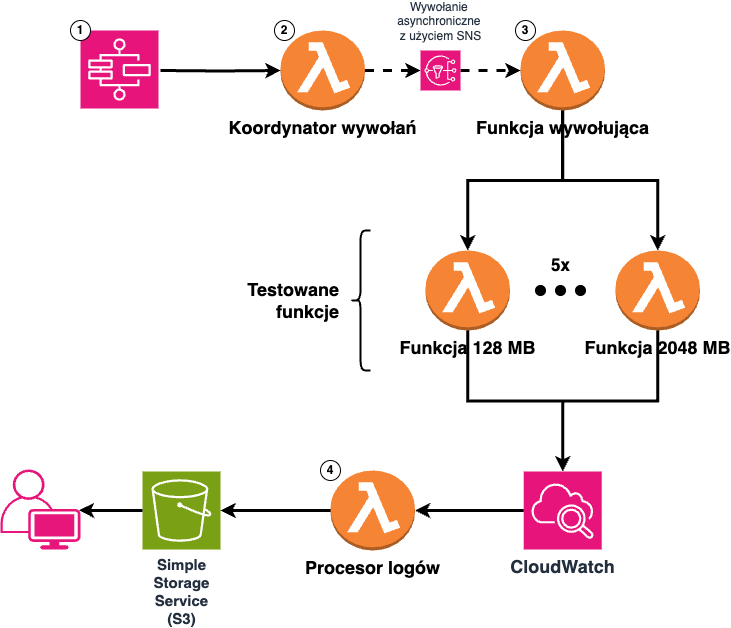
\includegraphics[width=1\textwidth]{charts/experiment-architecture.drawio.png}
    \caption{ Architektura środowiska badawczego [źródło:~opracowanie~własne]}
    \label{fig:experiment_architecture}
\end{figure}

    % \begin{enumerate}
    %     \item Cel badania, co mierzono i w jakiej konfiguracji (pamięć)
    %     \item Przygotowana funkcja:
    %     \begin{enumerate}
    %         \item Ogólna (mnożenie macierzy) + założenia
    %         \item Implementacja Java (Quarkus + GraalVM)
    %         \item Implementacja Kotlin (CommonMain + odpowiednio JVM, Native, JS)
    %     \end{enumerate}
    %     \item Budowanie i wdrożenie funkcji
    %     \begin{enumerate}
    %         \item Mierzenie czasu budowania
    %     \end{enumerate}
    %     \item Wykonywanie pomiarów (architektura)
    %     \item Obliczenie wydajności z wzoru oraz kosztów
    % \end{enumerate}
